%===============================================================================
% $Id: ifacconf.tex 19 2011-10-27 09:32:13Z jpuente $  
% Template for IFAC meeting papers
% Copyright (c) 2007-2008 International Federation of Automatic Control
%===============================================================================
\documentclass[a4paper]{ifacconf}

\usepackage{graphicx,amsmath,url}      % include this line if your document contains figures
\usepackage[round]{natbib}             % required for bibliography
%===============================================================================

%%%%%%%%%%%%%%%%%%%%%%%%%%%%%%%%%%%%%%%%%%%%%%%%%%%%%%%%%%%%%%%%%%%%%%%%%%%%%%%%%

\usepackage{newtxtext} % Same font for text and math
\usepackage{icomma} % Correct comma separation after numbers
\usepackage{newtxmath} % Same font for text and math
\usepackage{mathtools} % Required for paired delimiters
\DeclareUnicodeCharacter{FB01}{fi}

\usepackage{tabularx}
\newcolumntype{C}{>{\centering\arraybackslash}X}
\newcolumntype{R}{>{\flushright\arraybackslash}X}
\newcolumntype{L}{>{\flushleft\arraybackslash}X}
\usepackage{booktabs}
%\usepackage{cite}
\usepackage{url}

\usepackage[draft,nomargin,inline]{fixme}
% \usepackage[final]{fixme}

% fixme and changes setup
\fxusetheme{colorsig}
\fxsetup{inlineface=\footnotesize}
\FXRegisterAuthor{tfm}{atfm}{tfm}

\let\comment\undefined    % neutralize \comment command
\usepackage[draft]{changes}
% \usepackage[final]{changes}
\definechangesauthor[name={Tarcisio F. Maciel}]{tfm}
\setaddedmarkup{{\color{blue}#1}}
\setdeletedmarkup{{\color{red}\sout{#1}}}
%%%%%%%%%% 

\usepackage{pgfplots}
\pgfplotsset{compat=newest}

\usepackage{graphicx}

\usepackage{float}
\floatplacement{figure}{!htbp}

\usepackage[nolist]{acronym}


% USAR O PACOTE CLEVEREF PARA TODOS OS ELEMENTOS REFEENCIÁVEIS : ESTÁ BUGANDO!
%\usepackage{cleveref}
%\crefname{figure}{Figura}{Figuras}
%\crefname{table}{Tabela}{Tabelas}
%\crefname{equation}{}{}
%\crefname{section}{Seção}{Seções}s



\begin{acronym}
	\acro{LSTM}{\textit{Long Short-Term Memory}}
	\acro{RNA}{Rede Neural Artificial}
	\acroplural{RNA}[RNAs]{Redes Neurais Artificiais}
	\acro{RNR}{Rede Neural Recorrente}
	\acroplural{RNR}[RNRs]{Redes Neurais Recorrentes}
	\acro{MLP}{\textit{Multilayer Perceptron}}
	\acro{AR}{Autoregressivo}
	\acro{MA}{Média Móvel}
	\acro{ARIMA}{\textit{Autoregressive Integrated Moving Average}}
	\acro{ARMA}{\textit{Autoregressive Moving Average}}
	\acro{SARIMA}{\textit{Sazonal ARIMA}}
	\acro{MCG}{Modelo Num\'{e}rico de Circula\c{c}\~{a}o Geral}
	\acroplural{MCG}[MCGs]{Modelos Num\'{e}ricos de Circula\c{c}\~{a}o Geral}
	\acro{INMET}{Instituto Nacional de Meteorologia}
	\acro{FUNCEME}{Funda\c{c}\~{a}o Cearense de Meteorologia e Recursos H\'{i}dricos}
	\acro{NASA}{\textit{National Aeronautics and Space Administration}}
	\acro{IA}{Intelig\^{e}ncia Artificial}
	\acro{UFV}{Usina Fotovoltaica}
	\acroplural{UFV}[UFVs]{Usinas Fotovoltaicas}
	\acro{AP}{Aprendizagem Profunda}
	\acro{KDE}{\textit{Kernel Density Estimation}}
	\acro{ADF}{\textit{Augmented Dickey-Fuller}}
	\acro{ACF}{\textit{Autocorrelation Function}}
	\acro{PACF}{\textit{Partial ACF}}
	\acro{MK}{\textit{Mann-Kendall}}
	\acro{MAPE}{\textit{Mean Absolute Percentage Error}}
	\acro{MAE}{\textit{Mean Absolute Error}}
	\acro{RMSE}{\textit{Root Mean Square Error}}
\end{acronym}

\synctex=1


%%%%%%%%%%%%%%%%%%%%%%%%%%%%%%%%%%%%%%%%%%%%%%%%%%%%%%%%%%%%%%%%%%%%%%%%%%%%%%%%%




% ===============================================================
% Choose the language of the manuscript.
% If in English, choose 
% \def\portugues{0} 
%
% If in Portuguese or Spanish, choose
% \def\portugues{1} 
%
% Note that, if you are writing in Spanish, you need additional 
% adjusts in some parts of the text, which have been put in Portuguese only.
\def\portugues{1} 
% ===============================================================

% If the above line is commented, it is assumed manuscript in English:
\ifx\portugues\undefined
\def\portugues{0}
\fi


\if\portugues0
   \usepackage[english]{babel}
  \else
   \usepackage[spanish,brazil,english]{babel}
\fi

  

\usepackage[T1]{fontenc}
%\usepackage{inputenc}

\usepackage[utf8]{inputenc}

\usepackage{ae}


\if\portugues1
% =====================================================================
% =====================================================================
% If the manuscript is in Spanish, please change the texts adequatelly.
% You may also add other definitions in this part.
 \newtheorem{teorema}[thm]{{\em Teorema}}{ }
 \newtheorem{lema}[thm]{{\em Lema}}{ }
 \newtheorem{corolario}[thm]{{\em Corolário}}{ }
 \newenvironment{prova}{{\bf Prova.}}{ }
% ===============================================================
\fi

\begin{document}
	
	
\if\portugues1

% =====================================================================
% =====================================================================
% USE THIS PART IF THE TEXT IS IN PORTUGUES OR SPANISH
% =====================================================================
% If the manuscript is in Spanish, please change the texts adequately.
% =====================================================================
% 
\selectlanguage{brazil}
	
\begin{frontmatter}

\title{Predição de séries temporais de radiação solar utilizando modelos estatísticos e aprendizagem profunda na região de Quixeramobim - CE} 
% Title, preferably not more than 10 words.

%\thanks[footnoteinfo]{Reconhecimento do suporte financeiro deve vir nesta nota de rodapé.}


\author[First]{Raul Victor de O. Paiva} 
\author[Second]{ Tarcisio F. Maciel} 
\author[Third]{Wilker de O. Feitosa}
\author[Fourth]{Nícolas de A. Moreira}

\address[First]{Departamento de Engenharia de Teleinformática, Universidade Federal do Ceará, CE, (e-mail: raul.paiva@alu.ufc.br).}
\address[Second]{Departamento de Engenharia de Teleinformática, Universidade Federal do Ceará, CE (e-mail: maciel@gtel.ufc.br)}
\address[Third]{Departamento de Engenharia de Teleinformática, Universidade Federal do Ceará, CE (e-mail: wilker@gtel.ufc.br)}
\address[Fourth]{Departamento de Engenharia de Teleinformática, Universidade Federal do Ceará, CE (e-mail: nicolas.araujom@gmail.com)}

\selectlanguage{english}
\renewcommand{\abstractname}{{\bf Abstract:~}}
\begin{abstract}                % Abstract of not more than 250 words.
Weather forecasting is essential in the renewable energy sector, and it is indispensable to use climate informations such as air humidity, atmospheric pressure, temperature, wind speed and solar irradiation, which can be considered variables for forecasts in a certain region. 
In particular, there is a notable potential for the use of photovoltaic solar energy in the Brazilian Northeast due to the high solar irradiation levels in the region and, from the climatic time series, it is possible to train deep learning models that seek to predict the short and long term. This work aims to statistically analyze and predict a time series of total daily solar irradiation in the municipality of Quixeramobim, Ceará, through machine learning methods. The results obtained indicate that the models predict solar irradiance with low prediction error when compared to existing results in the literature. However, it is still necessary to investigate whether variables such as precipitation levels and temperature influence the predictions obtained in the study.

\vskip 1mm% não altere esse espaçamento
\selectlanguage{brazil}
{\noindent \bf Resumo}: A previsão do tempo é fundamental no setor de energias renováveis, sendo indispensável o uso de informações climáticas como umidade do ar, pressão atmosférica, temperatura, velocidade do vento e incidência de radiação solar, as quais podem ser consideradas variáveis para predições em uma determinada região. Em particular, há um notório potencial para o emprego de energia solar fotovoltaica no Nordeste brasileiro devido à grande incidência de radiação solar na região e, a partir das séries temporais climáticas, é possível treinar modelos de aprendizagem profunda que busquem prever a curto e longo prazo a irradiação solar. Este trabalho visa analisar estatisticamente e prever uma série temporal de incidência de radiação solar total diária no município de Quixeramobim, no Ceará, através do métodos de aprendizagem de máquina. Os resultados obtidos indicam que os modelos predizem a irradiação solar com erro de predição baixo quando comparado a resultados existentes na literatura. Contudo, é necessário ainda investigar se variáveis como níveis de precipitação e temperatura influenciam as predições obtidas no estudo.
\end{abstract}

\selectlanguage{english}


\begin{keyword}
solar irradiation; time series; data analysis; machine learning; data science

\vskip 1mm% não altere esse espaçamento
\selectlanguage{brazil}
{\noindent\it Palavras-chaves:} radiação solar; séries temporais; análise de dados; aprendizado de máquina; ciência de dados
\end{keyword}


\selectlanguage{brazil}


\end{frontmatter}
\else
% ===============================================================
% ===============================================================
% USE THIS PART IF THE TEXT IS IN ENGLISH
% ===============================================================
% ===============================================================
% 

\begin{frontmatter}

\title{Style for SBA Conferences \& Symposia: Use Title Case for
  Paper Title\thanksref{footnoteinfo}} 
% Title, preferably not more than 10 words.

\thanks[footnoteinfo]{Sponsor and financial support acknowledgment
goes here. Paper titles should be written in uppercase and lowercase
letters, not all uppercase.}

\author[First]{First A. Author} 
\author[Second]{Second B. Author, Jr.} 
\author[Third]{Third C. Author}


\address[First]{Faculdade de Engenharia Elétrica, Universidade do Triângulo, MG, (e-mail: autor1@faceg@univt.br).}
\address[Second]{Faculdade de Engenharia de Controle \& Automação, Universidade do Futuro, RJ (e-mail: autor2@feca.unifutu.rj)}
\address[Third]{Electrical Engineering Department, 
   Seoul National University, Seoul, Korea, (e-mail: author3@snu.ac.kr)}
   
\renewcommand{\abstractname}{{\bf Abstract:~}}   
   
\begin{abstract}                % Abstract of not more than 250 words.
These instructions give you guidelines for preparing papers for IFAC
technical meetings. Please use this document as a template to prepare
your manuscript. For submission guidelines, follow instructions on
paper submission system as well as the event website.
\end{abstract}

\begin{keyword}
Five to ten keywords, preferably chosen from the IFAC keyword list.
\end{keyword}

\end{frontmatter}
\fi

%===============================================================================
%===============================================================================
%===============================================================================


\section{Introdução}

Atualmente, o avanço tecnológico fornece recursos essenciais no auxílio à tomada de decisões em áreas diversas, como na Economia, Finanças e Gestão Ambiental. 

Em particular, para modelos de predição de séries temporais de dados climáticos, ainda existem limitações de processamento computacional pelo fato dos modelos numéricos clássicos, como os \acp{MCG}, serem muito complexos. De fato, os \acp{MCG} usam equações matemáticas representativas das leis físicas que regem os movimentos da atmosfera e as interações com os componentes do sistema climático e cuja solução depende de métodos numéricos de altíssima demanda computacional~\citep{Escobar2007, Sampaio2014}. A partir daí surge a necessidade de investigar novos métodos de predição de séries temporais climáticas, mais simples, com menor custo computacional, e que forneçam bons resultados, sejam eles estatísticos ou baseados em \acp{RNA}.

Neste contexto, a metodologia clássica usando o método \ac{ARIMA}, também conhecida como metodologia de Box-Jenkins, é uma abordagem comumente utilizada em predição de séries temporais, buscando expressar o comportamento futuro das séries baseado na variação estatística de seus dados no passado. O método~\ac{ARIMA} é considerado um método clássico devido à sua generalidade, podendo lidar com séries estacionárias ou não-estacionárias, sem ou com elementos sazonais \cite{Babai2013, Maddala2003}, sendo este último caso tratado pelo método \ac{SARIMA}.

Além dos modelos clássicos, \acp{RNA} vêm sendo empregadas com sucesso na predição de séries temporais por sua capacidade generalizada de aproximar funções não-lineares~\citep{Fernandes1996,Caloba2002,TorresJr2005}.

De fato, conforme~\cite{Mourao2019, Teixeira2019, Pereira2017, Ghaderi2017, Grover2015}, é viável treinar modelos preditivos de \ac{AP} a partir de séries temporais. A mesma conclusão é tomada em~\cite{Santos2013} em que se afirma que os instrumentos utilizados pelos meteorologistas foram se desenvolvendo e, com eles, a precisão das previsões do tempo foi melhorada substancialmente. Assim, o uso de \ac{AP} neste trabalho para predição de séries temporais climáticas encontra parte de sua justificativa.

Por outro lado, no contexto socioeconômico a participação das fontes fósseis na matriz energética mundial é de 79,5\% e, em 2017, 179 países tinham metas para aumentar essa participação em suas matrizes energéticas, um número que vem crescendo ao longo dos anos seguindo a introdução de novas políticas regulatórias para energias renováveis~\citep{Ren2018}. No caso dos grandes empreendimentos para geração elétrica a partir da energia solar fotovoltaica no Brasil, uma expansão, iniciada em 2014 com os primeiros projetos de \acp{UFV} vencedores de leilões de energia, é atribuída à redução dos custos de investimento, ao aumento da capacidade das usinas e à estimativa convidativa sobre a redução dos custos do empreendimento no horizonte de entrega da energia~\citep{Epe2018}.

Em~\cite{Mendes2017}, aponta-se que o aumento das usinas fotovoltaicas demandará dos responsáveis pela operação de sistemas elétricos a aplicação de ferramentas capazes de predizer a disponibilidade de recursos solares em curto prazo, em particular com o uso de \acp{RNA} na predição da radiação solar global. Lá destaca-se ainda que métodos de predição com \acp{RNA} podem ser aplicáveis a quaisquer regiões do Brasil, até mesmo àquelas em que não há estações de monitoramento suficientes, dada a capacidade de generalização das~\acp{RNA}.

Como pode ser visualizado na ~\ref{fig:mapa}, o nordeste brasileiro possui grande potencial para ampliação da energia fotovoltaica como matriz energética.No contexto regional, o Governo do Estado do Ceará tem favorecido e atraído investidores no setor das energias renováveis. Conforme~\cite{Epe2018}, no leilão A-4/2018 para contratação de projetos de energia solar, dentre 29 empreendimentos que foram contratados no Brasil, 14 deles são no Ceará, totalizando 390~MW de potência a ser instalada no estado. Deste modo, a justificativa e relevância de estudos como o conduzido neste trabalho são fortalecidas e o trabalho atual encontra-se portanto alinhado às iniciativas do Governo do Estado.

\begin{figure}
	\centering
	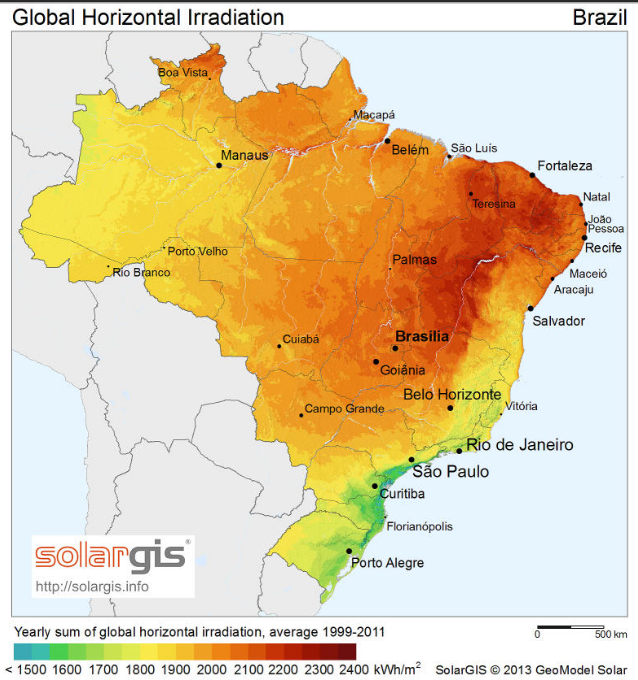
\includegraphics[width=0.8\columnwidth]{images/mapa.png}
	\caption{Irradiação solar no território Brasileiro. Média dos anos 1999 a 2011. Fonte:
		\protect\url{http://solargis.info}.}\label{fig:mapa}
\end{figure}

Através de técnicas de aprendizagem de máquina, é possível realizar um amplo estudo referente a séries temporais climáticas nas regiões do sertão central cearense, fornecendo predições de temperatura e incidência de radiação solar, por exemplo, em uma área específica do Ceará. Logo, este trabalho colabora com o desenvolvimento do setor de energia solar no Estado.

Neste trabalho foi abordado o treinamento de modelos preditivos para séries temporais de incidência de radiação solar a fim de mapear parte do potencial fotovoltaico da região de Quixeramobim-CE, utilizando \ac{AP} com o \ac{LSTM}, bem como os métodos estatísticos \ac{ARIMA} e \ac{SARIMA}.

O restante deste artigo está organizado como segue. A~\ref{sec:modelagem-series-rad} revisita brevemente as séries temporais, os métodos estatísticos \ac{ARIMA} e \ac{SARIMA}, e o método \ac{LSTM} de \ac{AP}. A~\ref{sec:resultados} apresenta a metodologia utilizada e os valores aplicados na parametrização dos estudos realizados, bem como realiza a discussão dos resultados obtidos através da análise do histograma, da densidade de probabilidade, das funções de autocorrelação e de autocorrelação parcial dos dados das séries temporais, além da aplicação de testes de estacionariedade e de tendência, e apresenta a comparação entre os métodos investigados. A~\ref{sec:conclusao} contém as principais conclusões obtidas a partir dos resultados obtidos e aponta algumas perspectivas de trabalhos futuros.

\section{Modelagem de séries temporais de radiação solar}\label{sec:modelagem-series-rad}

\subsection{Séries temporais climáticas e os modelos \acs{ARIMA}}\label{subsec:serie-temp-climaticas}
Séries de dados colhidos ao longo do tempo são chamadas de séries temporais e, quando se referem a dados climáticos, são chamadas de séries temporais climáticas. Séries temporais climáticas, como temperatura, pressão atmosférica, velocidade do vento e incidência de radiação solar, podem ser encontradas em bases de dados de órgãos competentes como o \ac{INMET} e a \ac{FUNCEME}, entre outros, subsidiando estudos que abrangem a temática de predições de fenômenos/eventos climáticos.

Uma série temporal $y_{t=1}^{T}, t = 1, \ldots, T$ é normalmente uma realização particular de um processo estocástico que pode ser representada como: %
\begin{equation}\label{eq1}
	y_{t=1}^{T} =  \{y_{1}, y_{2},  \ldots,  y_{t}, \ldots, y_{T-1}, y_{T}\}.
\end{equation} %

Através da análise dos dados contidos na série, diversas propriedades de interesse, como média, variância, periodicidade e estacionariedade, entre outras, dos dados podem ser extraídas a partir da aplicação de métodos estatísticos. Estas informações podem fornecer informações importantes sobre o fenômeno subjacente aos dados e auxiliar na tomada de decisões.

Como demonstrado em~\cite{Sampaio2014,Teixeira2019,Grover2015,Mendes2017}, a partir de séries temporais climáticas é possível construir modelos preditivos utilizando a modelagem clássica \ac{ARIMA} e suas variantes, assim como as \acp{RNA} de \ac{AP}. Além disso, é de conhecimento geral que modelos de \ac{AP} permitem avaliar uma quantidade maior de parâmetros, capturando os padrões ocultos nos dados das séries temporais tornando-se, portanto, uma ferramenta de grande potencial para a área.

Passando à breve discussão sobre os modelos \ac{ARIMA}, os mesmos são normalmente caracterizados por três parâmetros: %
\begin{itemize}
	\item $p$: o número de observações passadas inclusas no modelo, também conhecido como ``ordem de \textit{lag}", associadas ao componente \ac{AR} do método;
	\item $d$: o número de diferenças tomadas ou ``grau de diferenciação'', associadas à componente integrativa do método e que busca estabelecer estacionariedade;
	\item $q$: o tamanho da janela de média móvel ou ``ordem de média móvel'', associada a componente de \ac{MA} do método.
\end{itemize} %
Um modelo \ac{ARIMA} é usualmente representado pela notação $\text{\ac{ARIMA}}(p, d, q)$.

No contexto dos modelos \ac{ARIMA}, a metodologia Box-Jenkins investiga a autocorrelação entre valores da série em diferentes instantes sucessivos de tempo. Os padrões de autocorrelação, em geral, possibilitam identificar um ou vários modelos possíveis para a série temporal~\cite{Mehdi2010}.

De forma similar ao \ac{ARIMA}, o \ac{SARIMA} possui os parâmetros $p$, $d$, $q$ associados à parte não-sazonal do processo estocástico subjacente~\cite{Chen2007} e possui outros 4 parâmetros associados à parte sazonal do
mesmo: %
\begin{itemize}
	\item $P$: ordem da componente \ac{AR} sazonal;
	\item $D$: ordem de diferenças sazonais;
	\item $Q$: ordem da componente \ac{MA} sazonal;
	\item $s$: número de períodos referentes ao ciclo sazonal.
\end{itemize}
Em síntese, o modelo \ac{SARIMA} lida com a componente sazonal da série temporal e, por isso, o mesmo pode oferecer melhores resultados para dados que possuam sazonalidade inerente, como dados climáticos que são afetados pelas estações do ano.

Uma descrição mais aprofundada do método \ac{ARIMA} e suas variantes está fora do escopo deste trabalho, mas podem ser encontradas, por exemplo, em~\cite{Caloba2002, Mehdi2010, Chen2007}.

\subsection{\acs{RNR} e \ac{LSTM}}\label{subsec:lstm}

Conforme resume \cite{Teixeira2019}, as \acp{RNR} são representadas por uma realimentação na arquitetura padrão. O alcance dos valores utilizados para correção dos pesos é restrito, pois a influência da saída nas camadas ocultas decai exponencialmente à medida em que passa pelas conexões recorrentes da rede. Várias tentativas para resolver esta questão, conhecida como problema de dissipação de gradiente, foram abordadas durante os anos 90, e uma das soluções adotadas foi a criação das redes \ac{LSTM}.

A ideia central por trás da arquitetura \ac{LSTM} é uma atualização da memória $C_{n}$. O bloco de memória \textit{LSTM} está ilustrado na ~\ref{fig:lstm}.

\begin{figure}
	\centering
	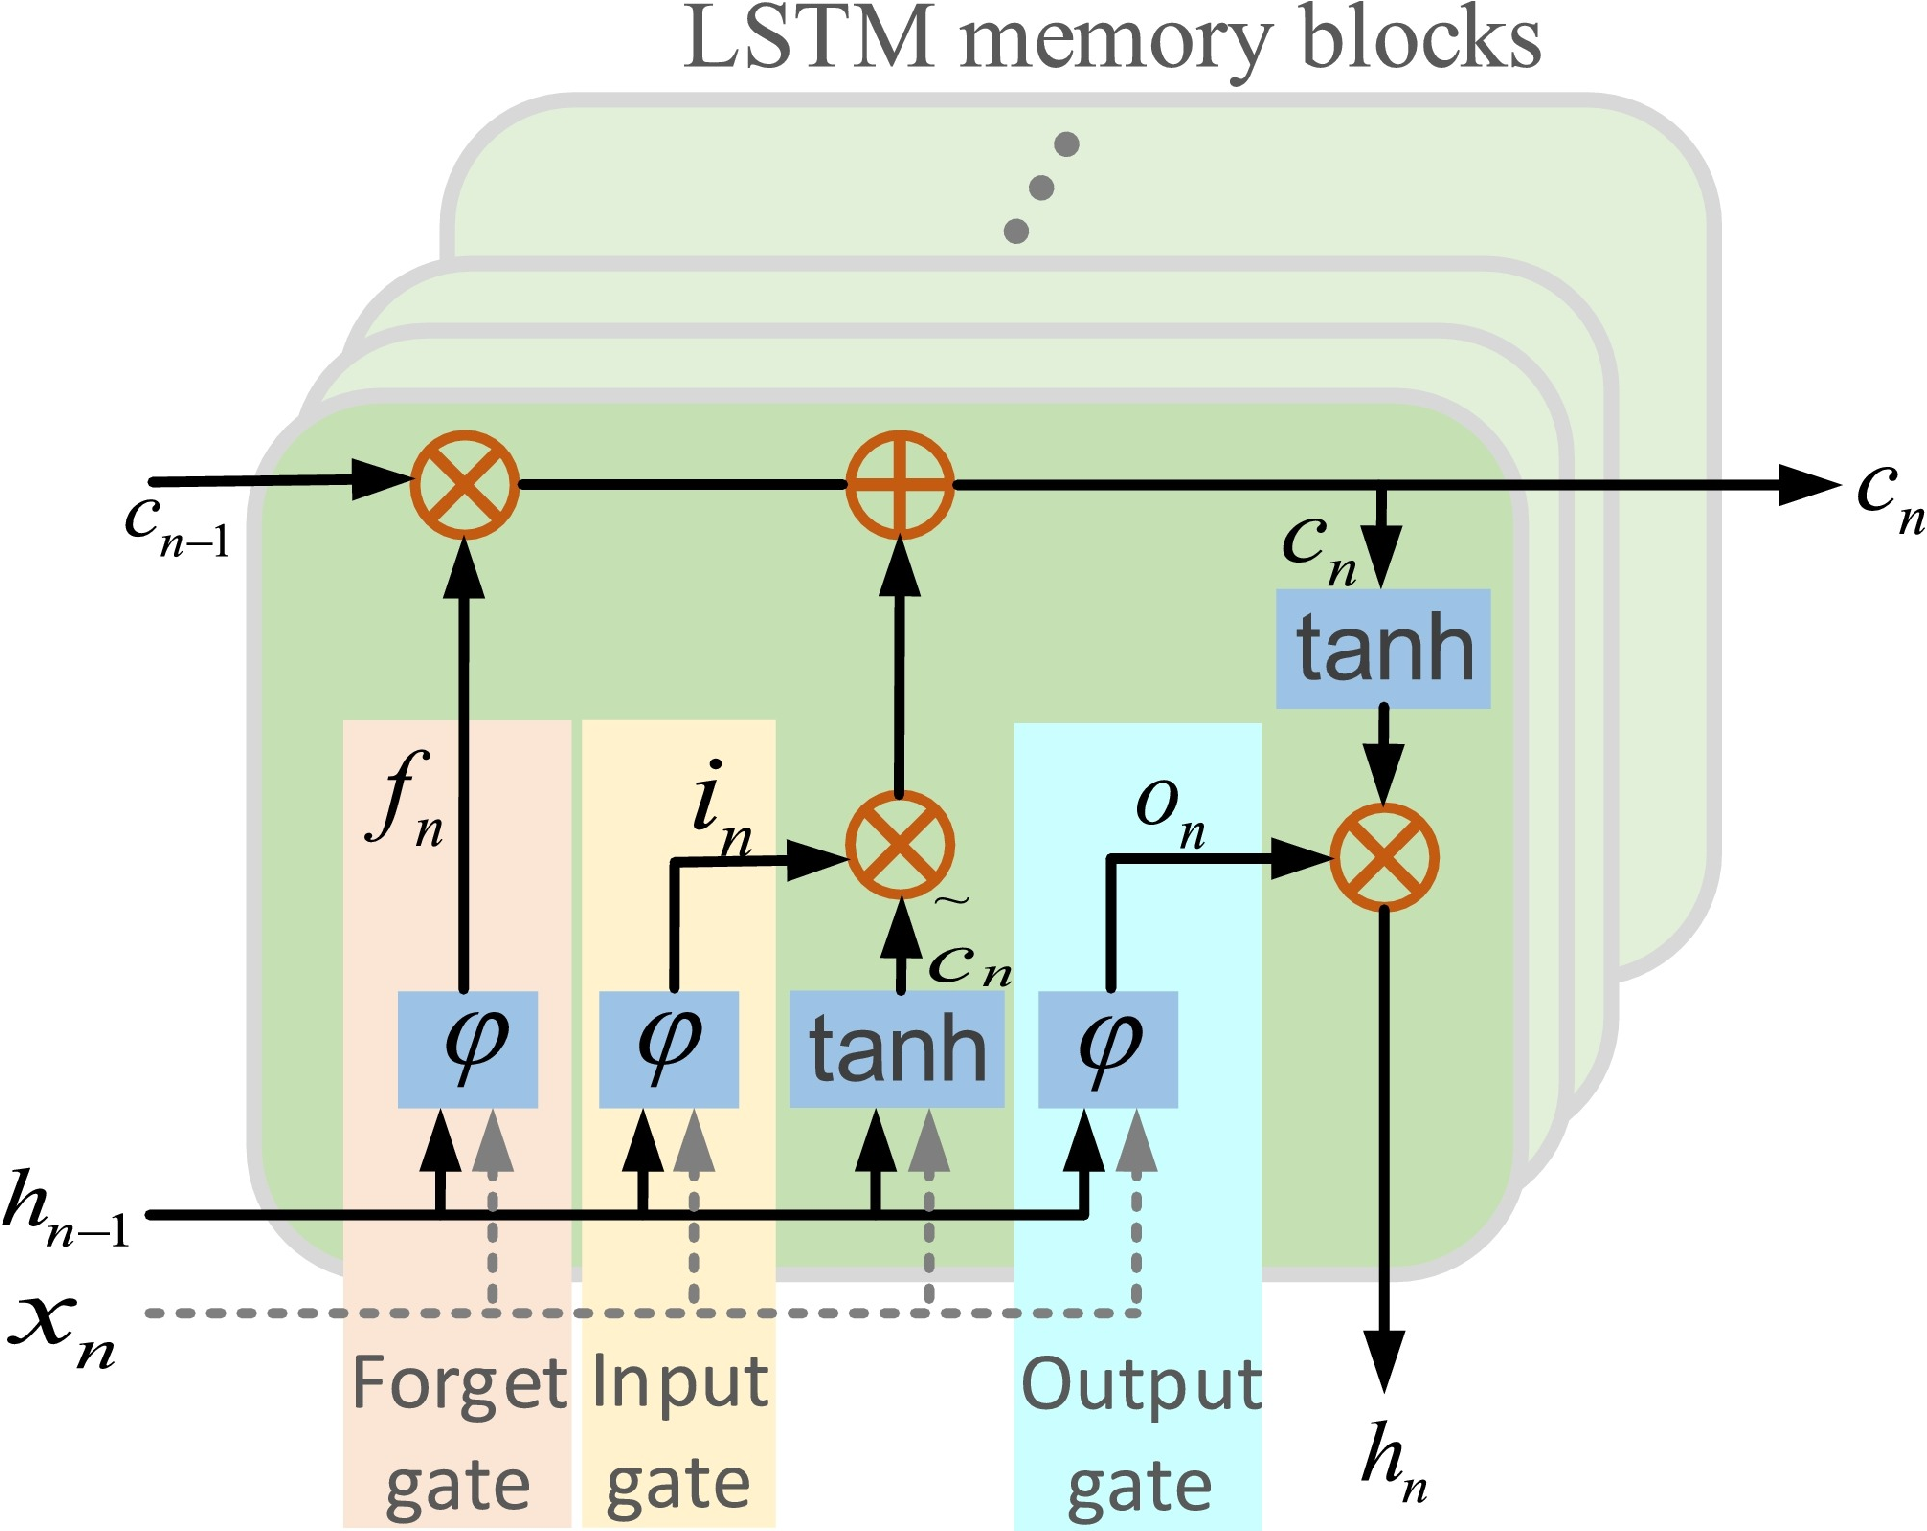
\includegraphics[width=0.9\columnwidth]{images/lstm-crop.pdf}
	\caption{Representação de uma célula LSTM~\cite{Rasmus2019}.}
	\label{fig:lstm}
\end{figure}

Agora o mesmo possui a capacidade de remover ou adicionar informações a esta memória em cada passo de tempo em uma sequência, controlada cuidadosamente por um \textit{forget gate} $f_{n}$ e um \textit{input gate} $i_{n}$, que empregam a mesma estrutura de uma rede neural de única camada com a função de ativação sigmóide~\cite{Rasmus2019}, e se relacionam com os demais de elementos (pesos, entradas, saídas, vieses, etc.) segundo a equação %
\begin{subequations}
	\begin{align}
		f            &= \varphi(b_{f} + \textbf{u}_{f}^{T}\textbf{x}_{n}+\textbf{w}_{f}^{T}\textbf{h}_{n-1}), \label{eq.FG}\\
		i_{t}         &= \varphi(b_{i} + \textbf{u}_{i}^{T}\textbf{x}_{n}+\textbf{w}_{i}^{T}\textbf{h}_{n-1}). \label{eq.IG}
	\end{align}
\end{subequations} %

Os autores em~\cite{Rasmus2019} ressalvam que $\textbf{x}_{n}$ é a sequencia de entrada no passo de tempo $n$, e
$\textbf{h}_{n-1}$ é o vetor de saída da \ac{LSTM} no passo de tempo passado. Os parâmetros $\textbf{u}_{i}$,
$\textbf{w}_{i}$, $\textbf{u}_{f}$ e $\textbf{w}_{f}$ são as entradas e os vetores de peso recorrentes do \textit{input}
e \textit{forget gates}, respectivamente, em que os \textit{b's} são todos os termos dos vieses. Os autores ainda
ressaltam que a função de ativação sigmoide é responsável por controlar o quanto de cada componente deve passar. Ainda
segundo ~\cite{Rasmus2019}, a memória $C_{n}$ é atualizada esquecendo parcialmente a memória existente e adicionando
um novo conteúdo de memória $C_{\tilde{n}}$ dado por %
\begin{subequations}
	\begin{align}
		C_{n} & = f_{n}C_{n-1}+i_{n}\tilde{C}_{n}, \label{eq.C}\\
		\tilde{C}_{n}  &= \tanh(b_{i} + \textbf{u}_{c}^{T}\textbf{x}_{n}+\textbf{w}_{c}^{T}\textbf{h}_{n-1}). \label{eq.C_tilde}
	\end{align}
\end{subequations}

O \textit{output gate} $o_{n}$ possui estrutura familiar à do \textit{input} e \textit{forget gate}. A saída da \ac{LSTM} é dada por %
\begin{subequations}
	\begin{align}
		h_{n} & = o_{n}\tanh(C_{n}) \label{eq.h}, \\
		o_{n}  &= \tanh(b_{o} + \textbf{w}_{o}^{T}\textbf{x}_{n}+\textbf{u}_{o}^{T}\textbf{h}_{n-1}), \label{eq.O}
	\end{align}
\end{subequations}
em que os termos $\textbf{u}_{o}$ e $\textbf{w}_{o}$ são os vetores de peso de entrada e recorrente do \textit{output gate}, respectivamente~\cite{Rasmus2019}. Uma análise mais detalhada de \acp{RNR}, \ac{LSTM}, e suas aplicações, foge ao escopo deste trabalho, sendo o leitor interessado em descrições mais aprofundadas direcionado às referências~\citep{Rasmus2019,Ghaderi2017,Pereira2017}.

\section{Análise dos Resultados}\label{sec:resultados}

Nos estudos realizados neste trabalho utilizaram a linguagem de programação \texttt{Python} para a modelagem e análise dos dados. Em particular, o método \ac{ARIMA} foi acessado a partir da biblioteca \texttt{statsmodels} \citep{Seabold_statsmodels2010}. Para a otimização dos parâmetros, o método \textit{walk-forward} foi utilizado. Os parâmetros $p$ e $q$ dos modelos \ac{ARIMA} e \ac{SARIMA} foram determinados através de uma busca direta nos intervalos $0 \leq p \leq 9$ e $0 \leq q \leq 4$, respectivamente, enquanto que $d = 0$ foi adotado não tendo sido portanto diferenciada a série.

A série de radiação solar coletada na região de Quixeramobim foi acessada na base de dados públicos da página oficial do \ac{INMET}. A~\ref{fig:decomposicao} apresenta a série temporal completa, com 1827 observações, juntamente com a decomposição da série nas componentes de tendência, sazonalidade e resíduo.
\begin{figure}
	\centering
	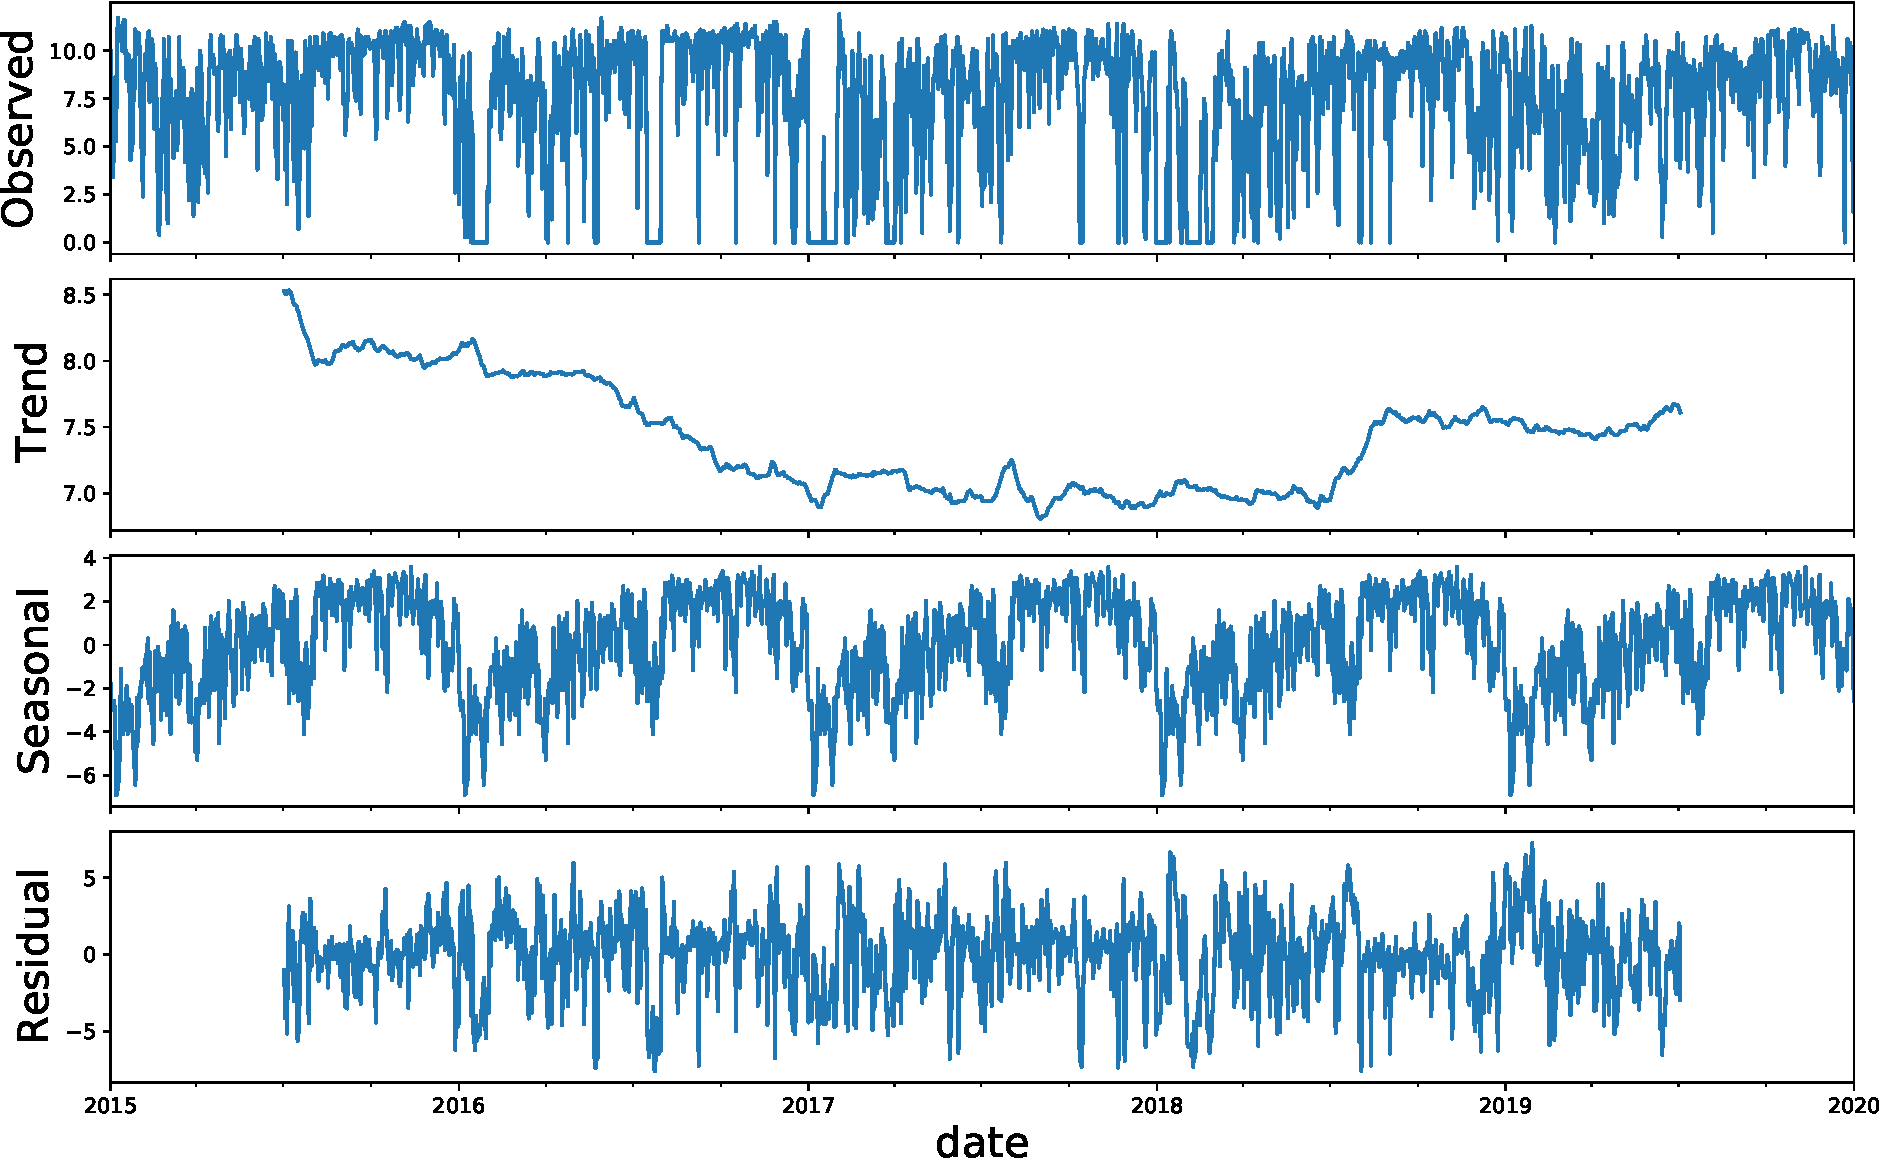
\includegraphics[width=0.9\columnwidth]{images/decomposicao.pdf}
	\caption{Decomposição da série completa nas componentes de tendência, sazonalidade e erro (resíduo).}\label{fig:decomposicao}
\end{figure}

A decomposição foi realizada a partir da função \texttt{statsmodels.tsa.seasonal.seasonal\_decompose} do módulo \texttt{statsmodels} em \texttt{Python}. É possível observar uma tendência crescente em determinadas épocas e decrescente em outras. A sazonalidade, com frequência equivalente a 365 pontos, apresenta uma série que possui um padrão intrínseco. É possível observar o extenso nível de erro a partir do gráfico residual.

Na~\ref{fig:hist_dist}, nota-se no histograma e distribuição de densidade de probabilidade que a maior incidência de radiação está entre 9 a 11~KJ/m$^{2}$.  
\begin{figure}
	\centering
	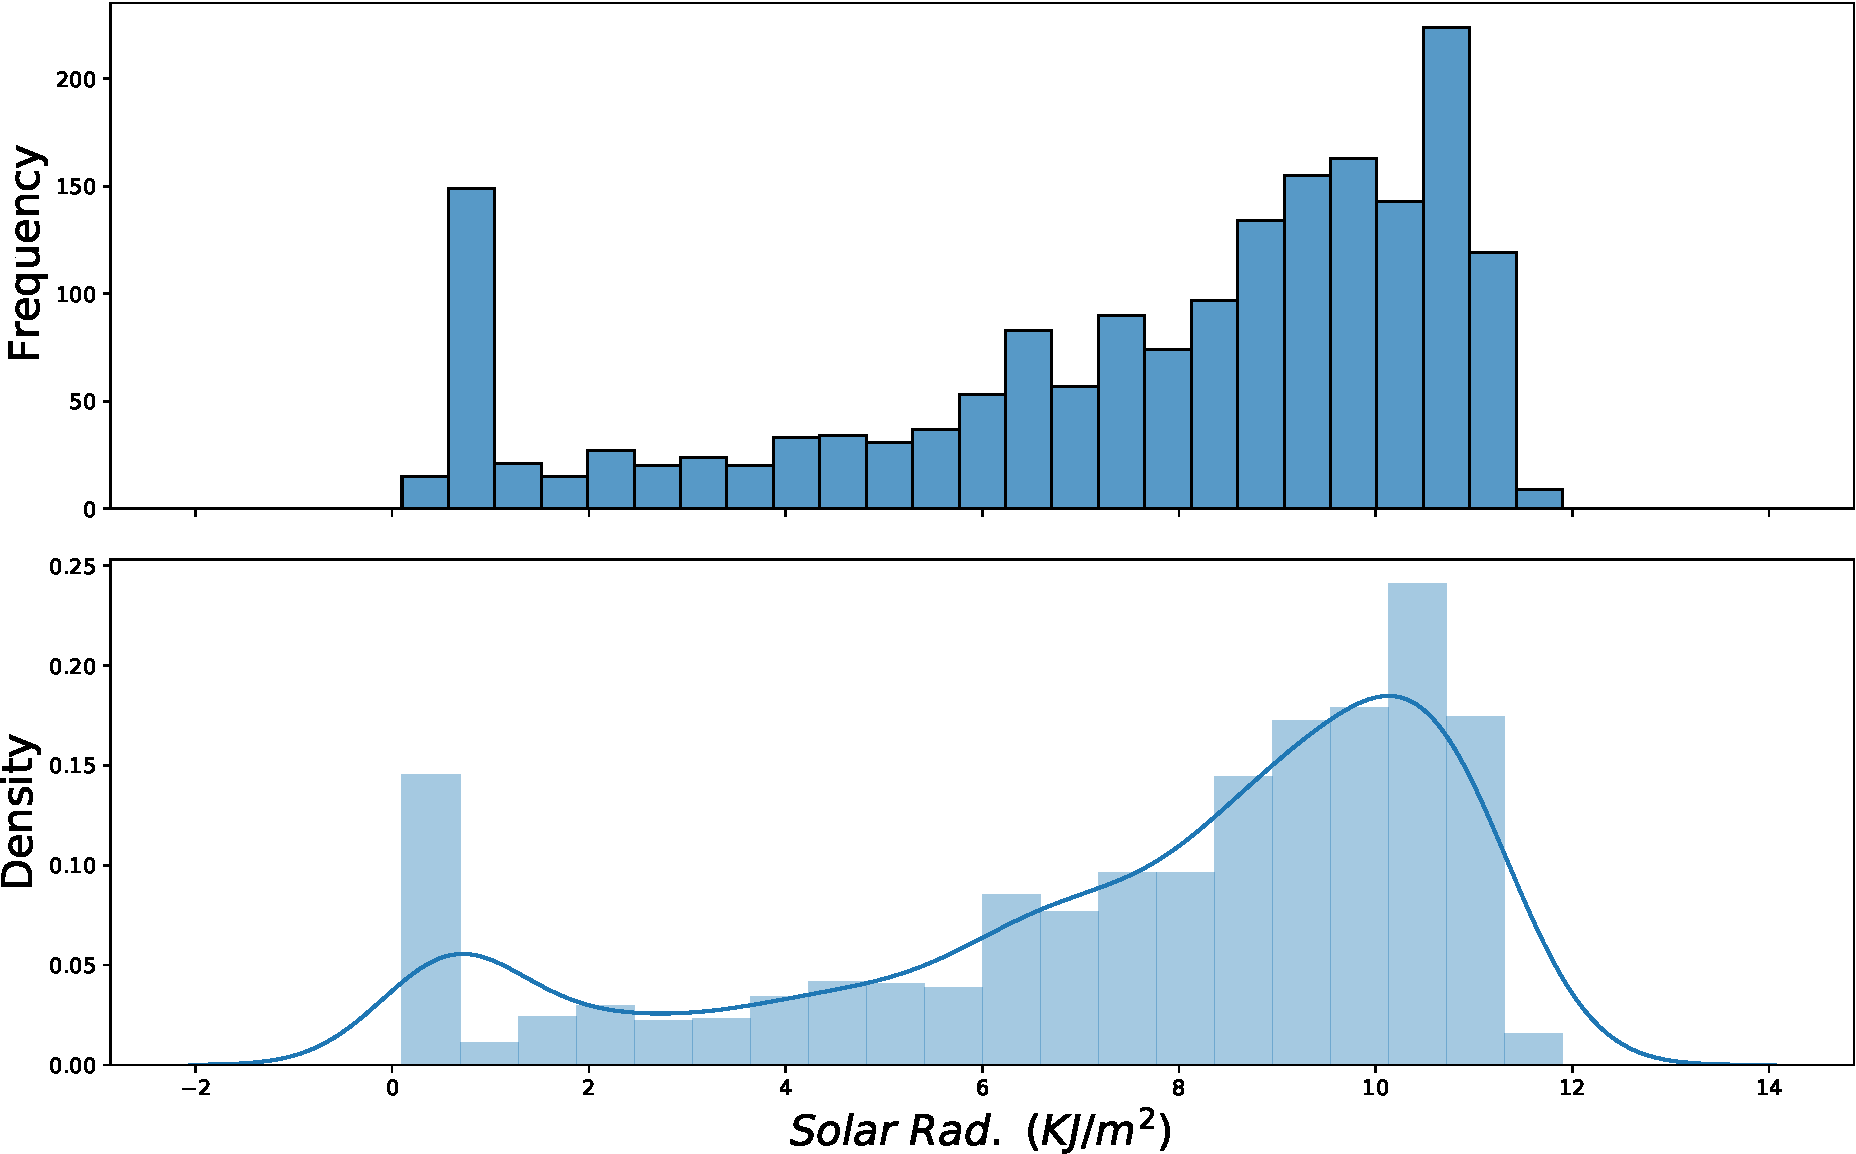
\includegraphics[width=0.9\columnwidth]{images/hist_dist.pdf}
	\caption{Histograma e densidade de probabilidade da série de radiação solar.}
	\label{fig:hist_dist}
\end{figure}

As análises indicadas acima são importantes para melhor compreensão dos dados em questão. Todavia, é necessário avaliar os parâmetros necessários para iniciar a modelagem com os métodos \ac{ARIMA}. As análises da \ac{ACF} e \ac{PACF} pode ajudar nesta avaliação. 
%{\color{red}QUAL FOI O NÍVEL DE SIGNIFICÂNCIA EXATO QUE VOCÊ USOU? 0.5 DE CORRELAÇÃO RESIDUAL, $1/e$, 0.1?}
Na~\ref{fig:ACF_PACF}, pode-se notar que a \ac{ACF}, com nível de significância equivalente a $5\%$, revela o intervalo de confiança até por volta de 20 \textit{lags}, pois conforme os dados de comparação são afastados, o resultado da correlação se aproxima de 0. Verifica-se na \ac{PACF} uma significância em até 3 lags. Estas avaliações são importantes para a determinação inicial dos parâmetros do modelo \ac{ARIMA}, uma vez que os \textit{lags} na \ac{ACF} ajudam a definir o parâmetro $q$ da média móvel, equanto os da \ac{PACF} definem o $p$ da autorregressão.

\begin{figure} %ACF e PACF
	\centering
	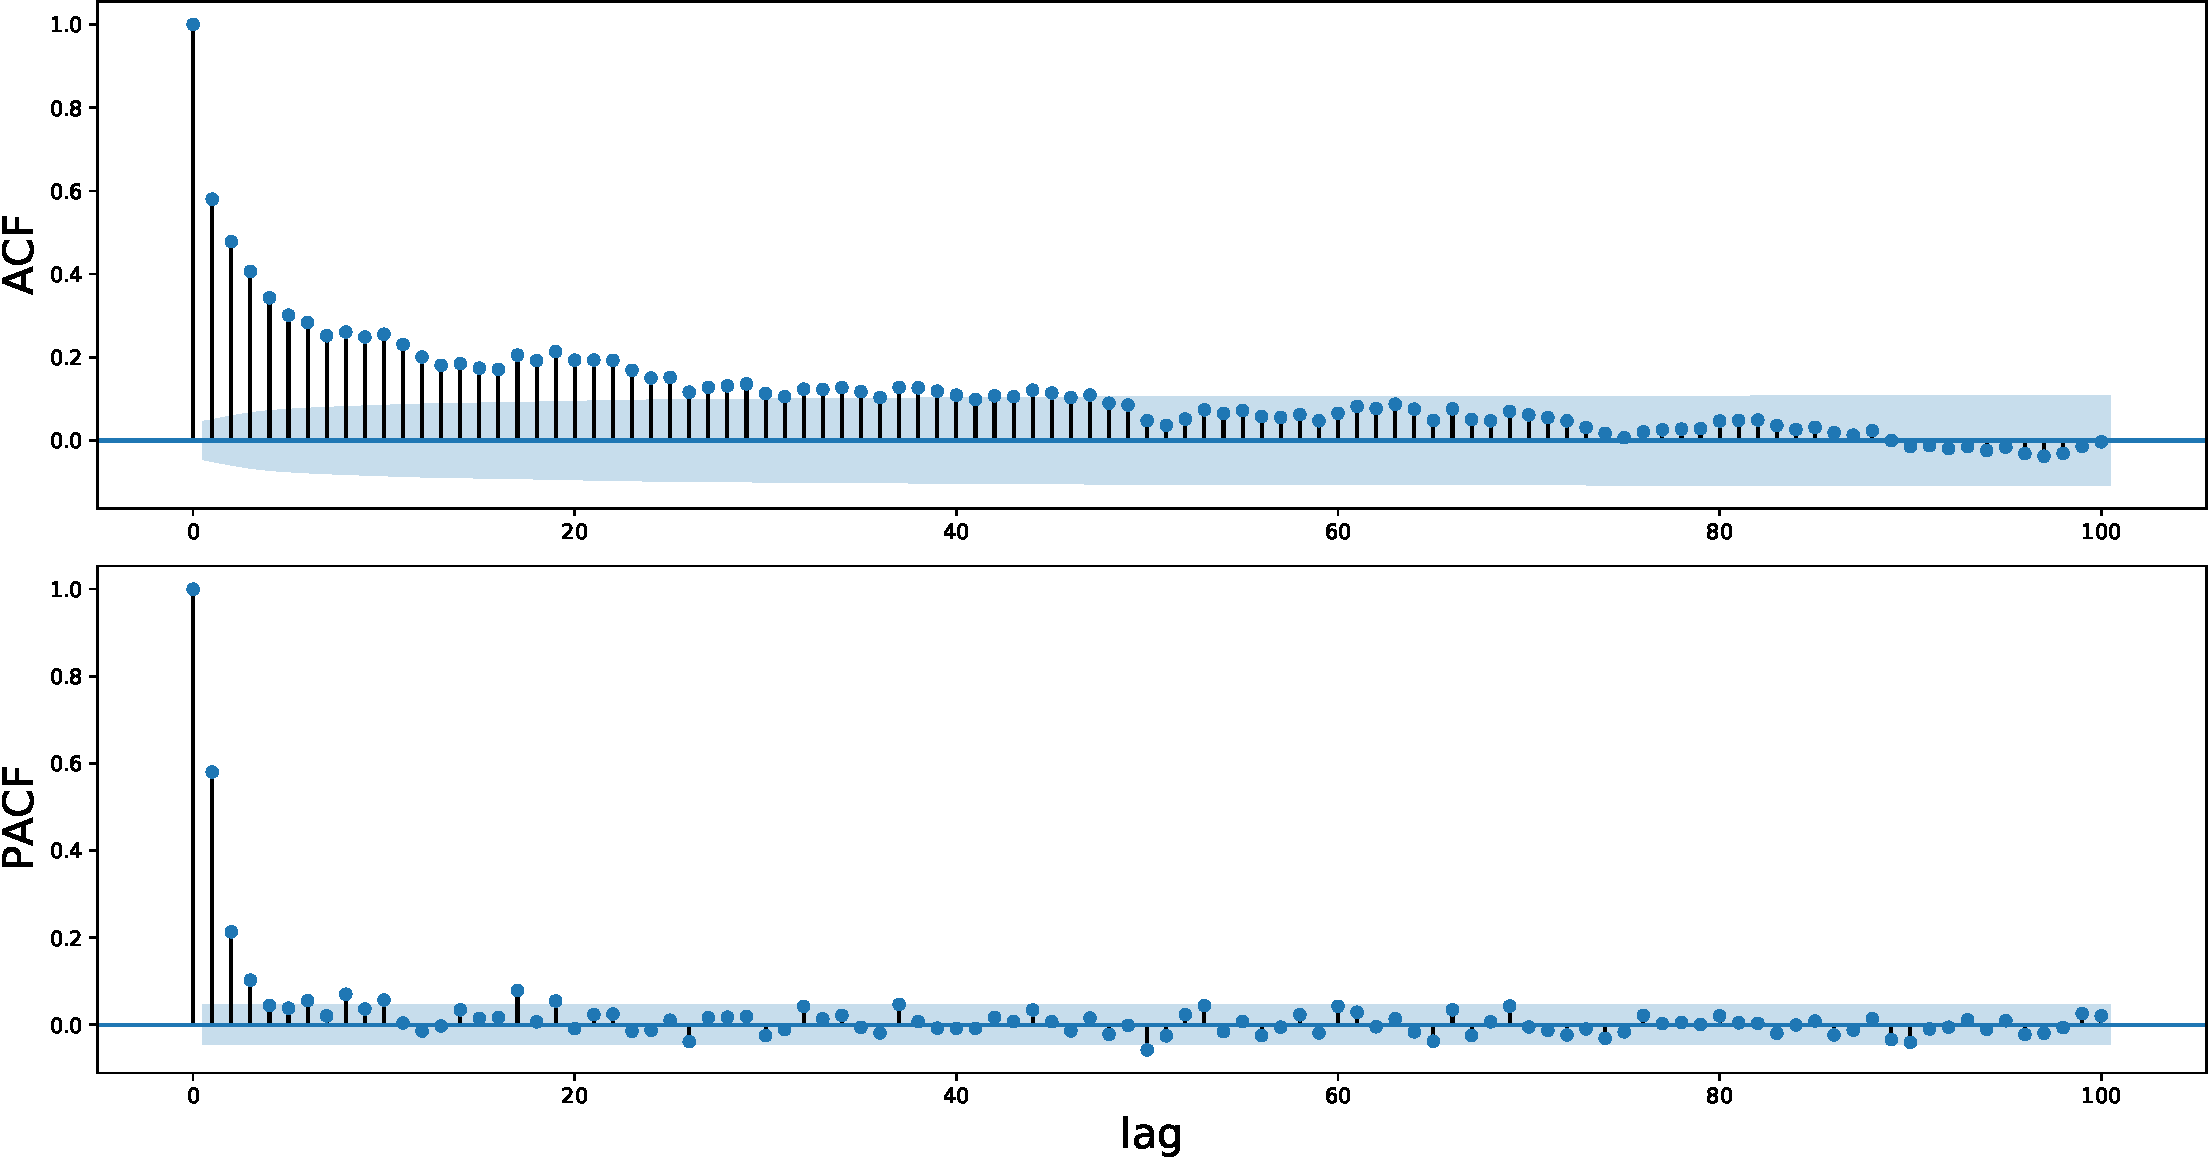
\includegraphics[width=0.9\columnwidth]{images/acf_pacf.pdf}
	\caption{Funções de autocorrelação e autocorrelação parcial.}\label{fig:ACF_PACF}
\end{figure}

Ainda sobre os parâmetros do modelo \ac{ARIMA}, também é possível verificar inicialmente se é necessário utilizar algum grau de diferenciação ($d$) na série, para isto, o teste \ac{ADF} fornece as respostas necessárias. Ao realizar a análise de séries temporais, é necessário verificar a estacionariedade~\cite{Vasconcellos2000}. Portanto, teste \ac{ADF} foi realizado em que a hipótese nula foi testada para a investigação da estacionariedade, com nível de significância equivalente a $5\%$. Para análise de tendência, culminando em um estudo mais apurado, foi realizado o teste de \ac{MK}, pois segundo~\cite{Goossens1986} o teste de \ac{MK} é o método mais apropriado para analisar mudanças climáticas, além de permitir a detecção e localização aproximada do ponto inicial de determinada tendência.

\begin{table}
	\centering
	\caption{Resultados dos testes  \ac{ADF} e \ac{MK} do conjunto de dados de Quixaramobim.}
	\begin{tabularx}{\columnwidth}{ccCCC} 
		\toprule
		Série        & \ac{ADF} & Valor $p$             & \ac{MK}               & Valor $p$ \\
		\midrule
		Original     & -5,70    & 7,60$\times 10^{-7}$  & -1,95$\times 10^{-4}$ & 1,73$\times 10^{-2}$   \\ %\midrule
		Diferenciada & -15,90   & 7,80$\times 10^{-29}$ & 0,00                  & 9,93$\times 10^{-1}$   \\
		\bottomrule
	\end{tabularx}
\end{table}
O teste \ac{MK} retornou tendência decrescente para a série original, como pode ser observado na \ref{fig:decomposicao}, e nula para a série diferenciada com ordem 1.

{\color{purple}PAREI AQUI. FAZER O ELO ENTRE A "POSSIBILIDADE DA MODELAGEM" E "SEPARAÇÃO DE TREINO E TESTE"! }
Com tudo, tendo em vista a análise prévia da série de radiação solar no município de Quixeramobim, foi possível criar modelos preditivos com os clássicos \ac{ARIMA} e \ac{SARIMA}, e com a \ac{LSTM} de \ac{AP}. Para isto, foi... . Na \ref{fig:train_test} abaixo, segue a divisão da base de treino e teste. A divisão da base de dados consta em $80\%$
de treino, que equivale ao período de janeiro de 2015 a dezembro de 2018.
\begin{figure} 
	\centering
	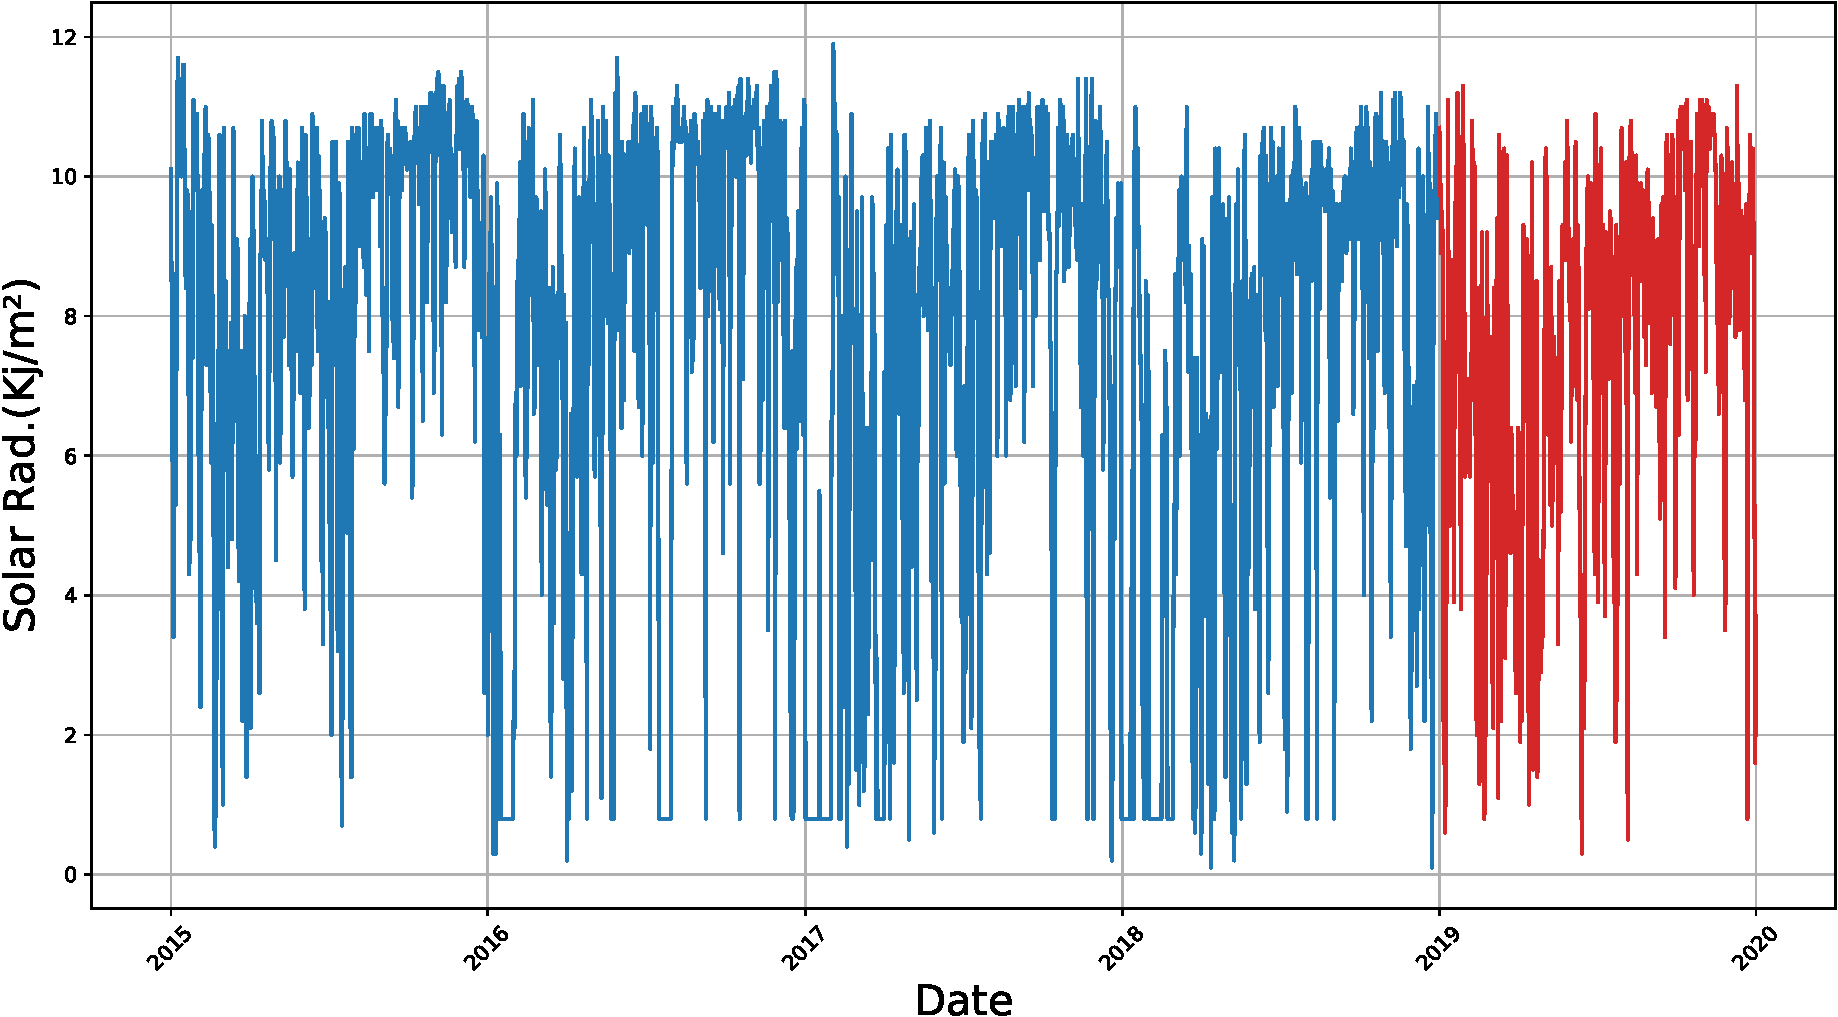
\includegraphics[width=0.9\columnwidth]{images/train_test.pdf}
	\caption{Divisão da base de treino e teste.}\label{fig:train_test}
\end{figure}

%PRONTO. A PARTIR DAQUI EU MODIFICO AO LONGO DO RESTO DA SEMANA - by: Raul


\begin{figure} 
	\centering
	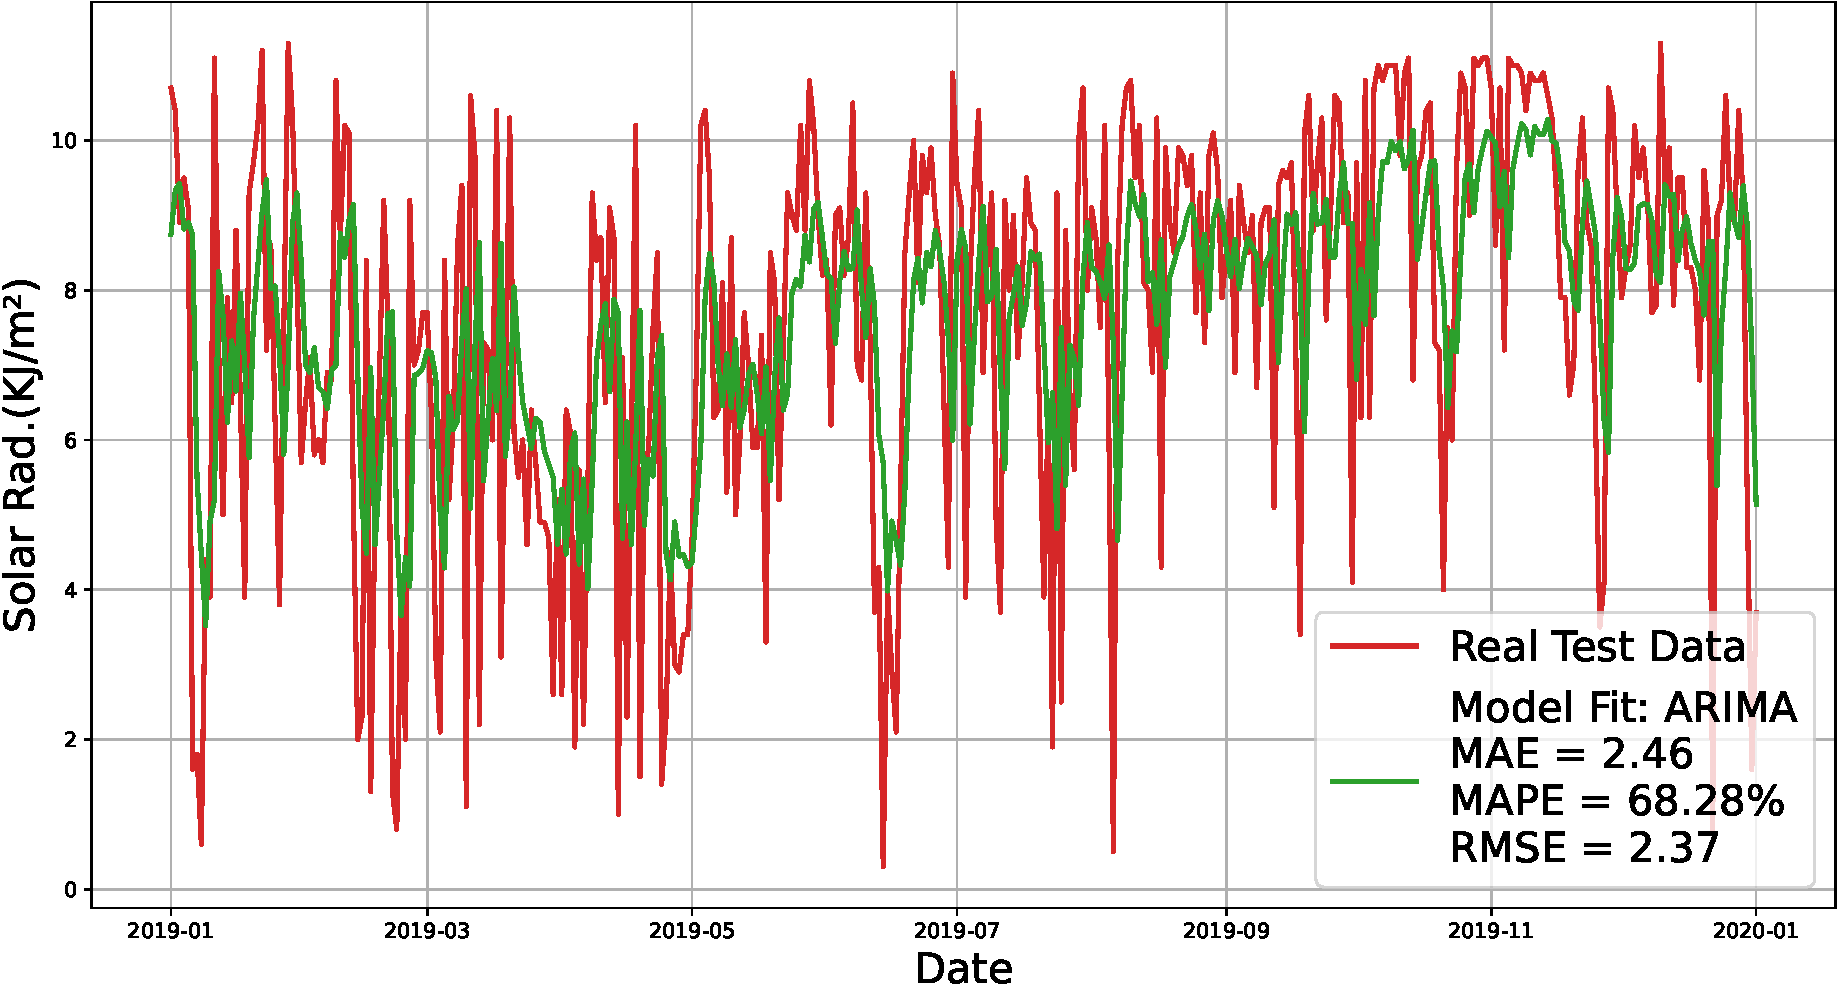
\includegraphics[width=0.9\columnwidth]{images/ARIMA_forecast.pdf}
	\caption{Predição com o modelo \ac{ARIMA}(5, 0, 3).}\label{fig:arima_forecast}
\end{figure}

\begin{figure} 
	\centering
	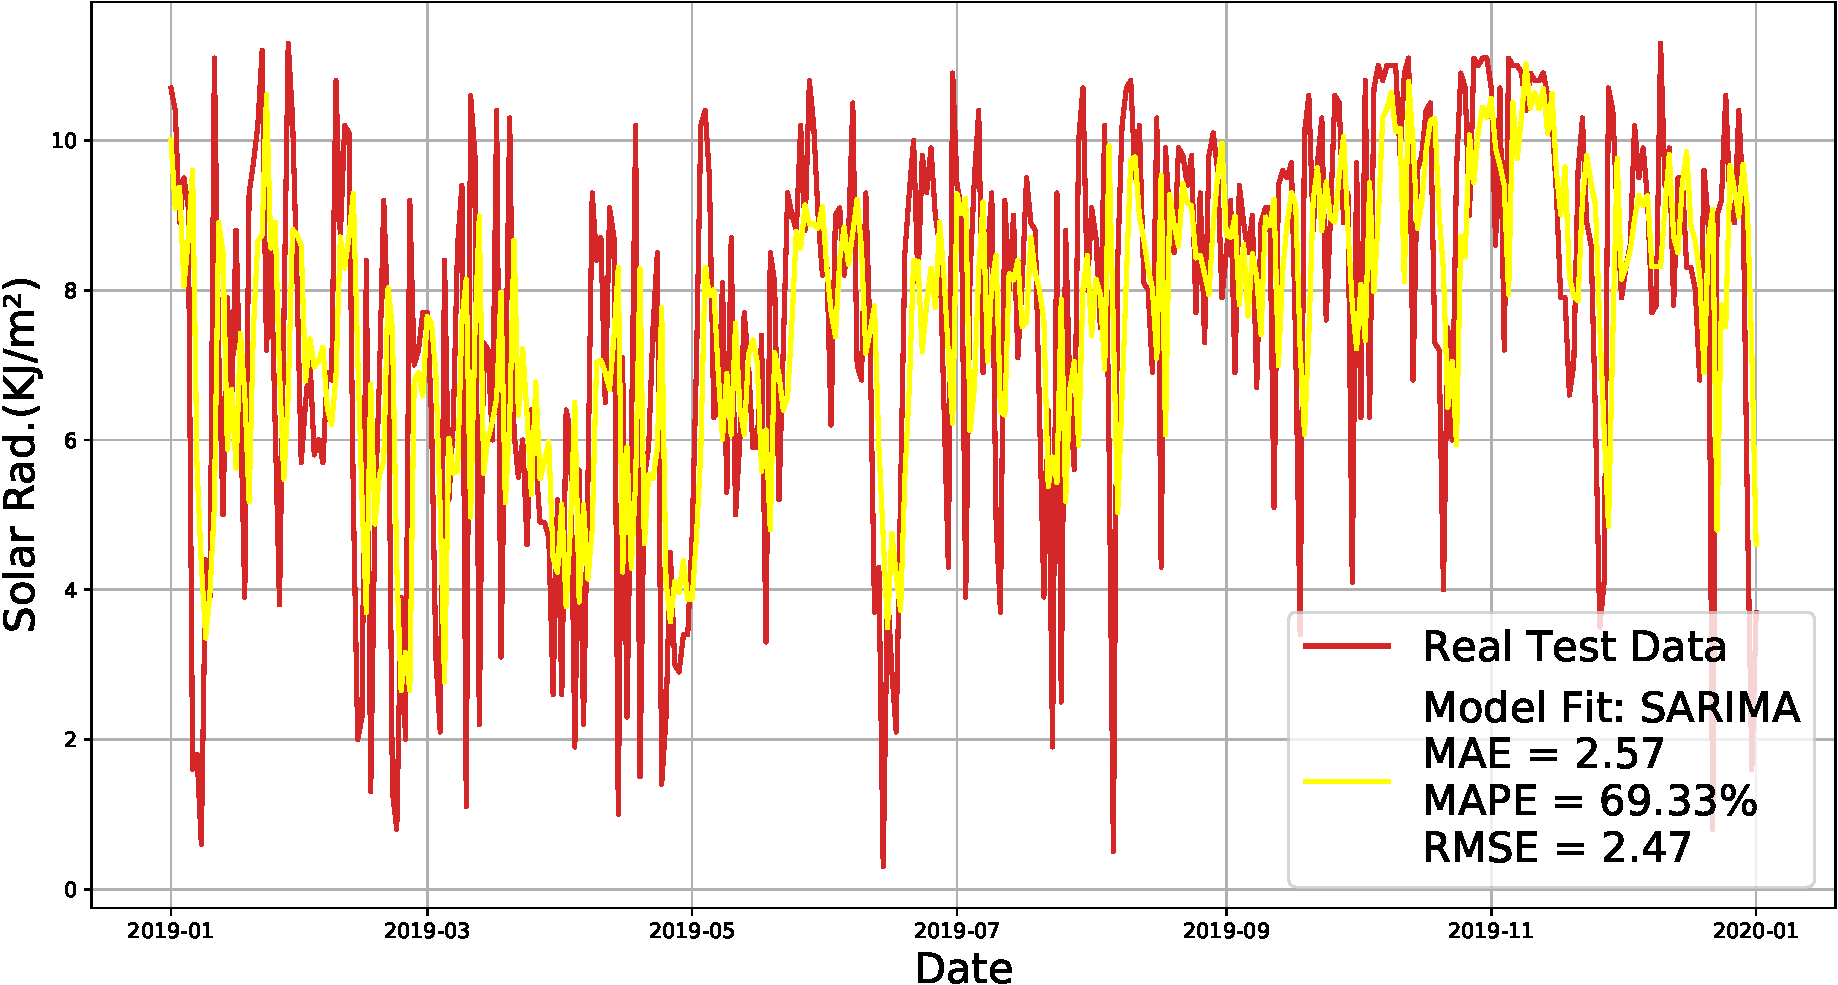
\includegraphics[width=0.9\columnwidth]{images/SARIMA_forecast.pdf}
	\caption{Predição com o modelo \ac{SARIMA}(5, 0, 3)(4, 0, 4, 12).}\label{fig:sarima_forecast}
\end{figure}

\begin{figure} 
	\centering
	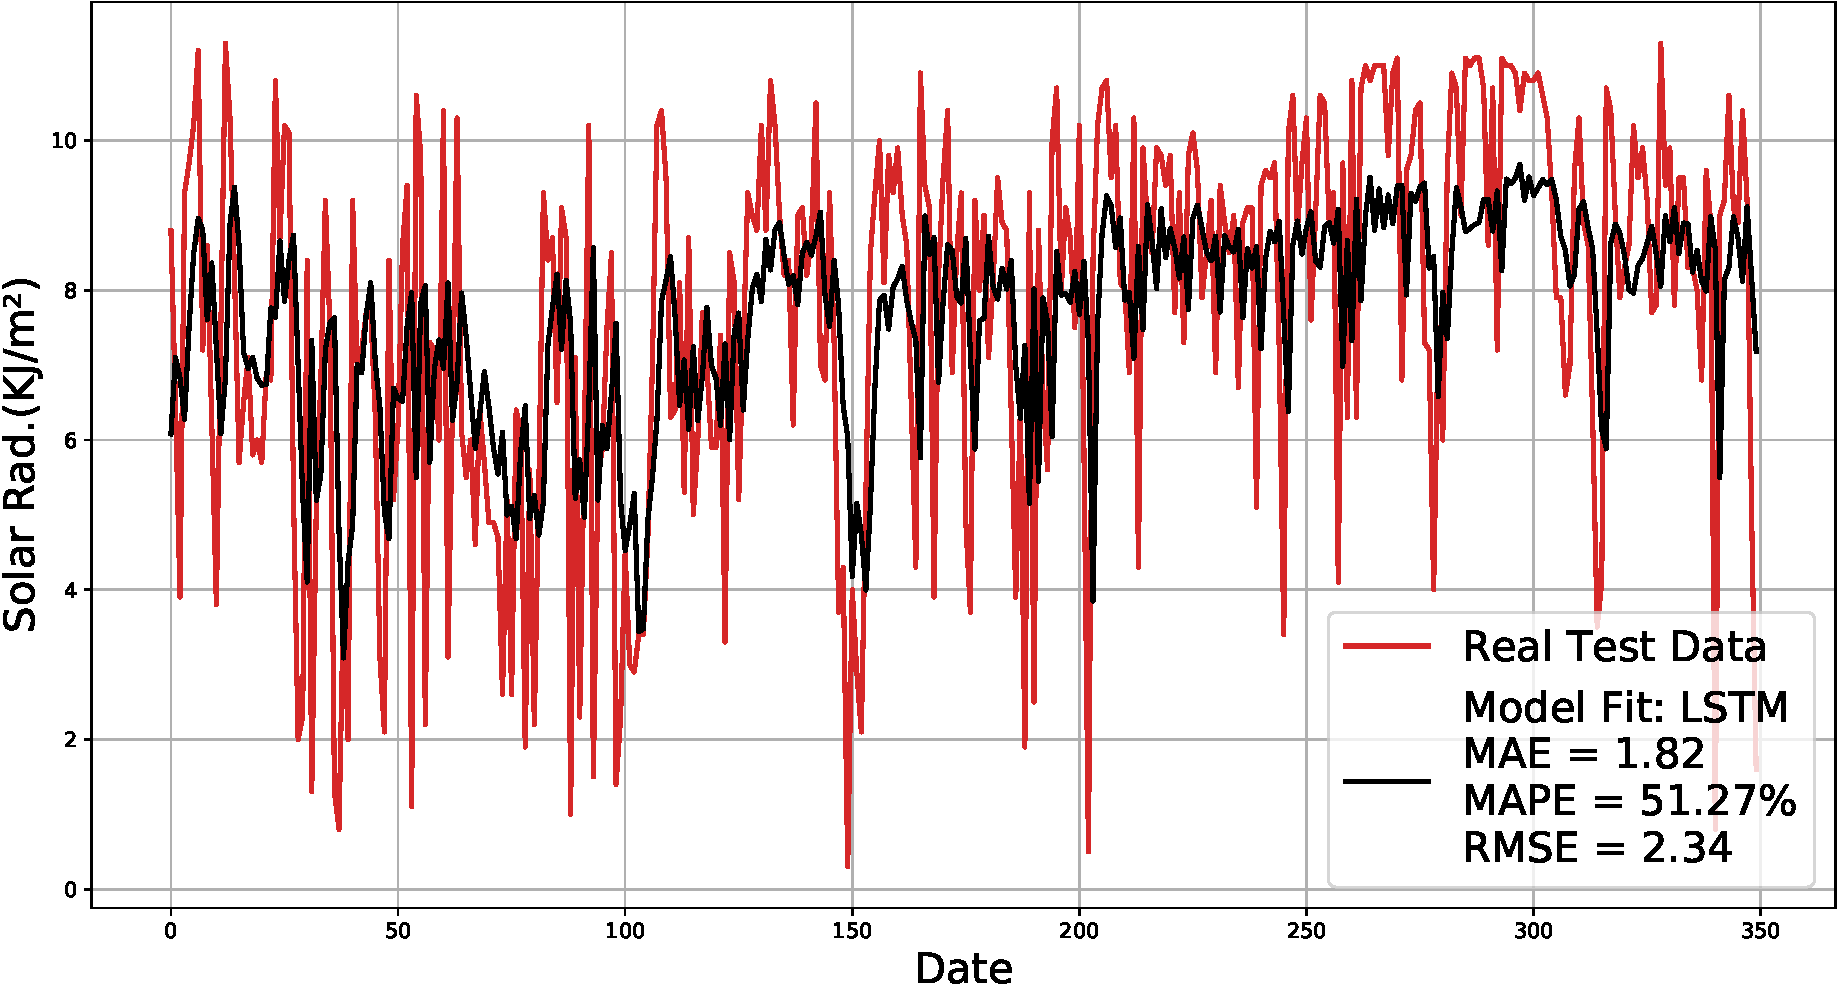
\includegraphics[width=0.9\columnwidth]{images/LSTM_forecast.pdf}
	\caption{Predição com o modelo \ac{LSTM}.}\label{fig:lstm_forecast}
\end{figure}

\begin{table}
	\centering
	\begin{tabularx}{\columnwidth}{CCCC}
		\cline{2-4}
		& \multicolumn{3}{c}{Base de Teste} \\ \midrule
		MODELOS         & MAPE (\%)  & MAE   & RMSE (kJ/m2) \\ \midrule
		ARIMA 			& 68.28      & 2.46  & 2.38         \\
		SARIMA          & 69.33      & 2.47  & 2.57         \\
		LSTM            & 51.27      & 1.82  & 2.34         \\ \bottomrule
	\end{tabularx}
\end{table}

\section{Conclusão}\label{sec:conclusao}


\section*{Agradecimentos}
Coloque aqui seus agradecimentos. 

\bibliography{ifacconf}             % bib file to produce the bibliography
                                                     % with bibtex (preferred)
                                                   
%\begin{thebibliography}{xx}  % you can also add the bibliography by hand

%\bibitem[Able(1956)]{Abl:56}
%B.C. Able.
%\newblock Nucleic acid content of microscope.
%\newblock \emph{Nature}, 135:\penalty0 7--9, 1956.

%\bibitem[Able et~al.(1954)Able, Tagg, and Rush]{AbTaRu:54}
%B.C. Able, R.A. Tagg, and M.~Rush.
%\newblock Enzyme-catalyzed cellular transanimations.
%\newblock In A.F. Round, editor, \emph{Advances in Enzymology}, volume~2, pages
%  125--247. Academic Press, New York, 3rd edition, 1954.

%\bibitem[Keohane(1958)]{Keo:58}
%R.~Keohane.
%\newblock \emph{Power and Interdependence: World Politics in Transitions}.
%\newblock Little, Brown \& Co., Boston, 1958.

%\bibitem[Powers(1985)]{Pow:85}
%T.~Powers.
%\newblock Is there a way out?
%\newblock \emph{Harpers}, pages 35--47, June 1985.

%\bibitem[Soukhanov(1992)]{Heritage:92}
%A.~H. Soukhanov, editor.
%\newblock \emph{{The American Heritage. Dictionary of the American Language}}.
%\newblock Houghton Mifflin Company, 1992.

%\end{thebibliography}

%\appendix
%\section{Sumário da gramática sânscrita}    % Each appendix must have a short title.
%\section{Algum vocabulário maia}              % Sections and subsections are supported  
%                                                                         % in the appendices.
\end{document}
